%\begin{sidewaysfigure}
%  \begin{center}
%  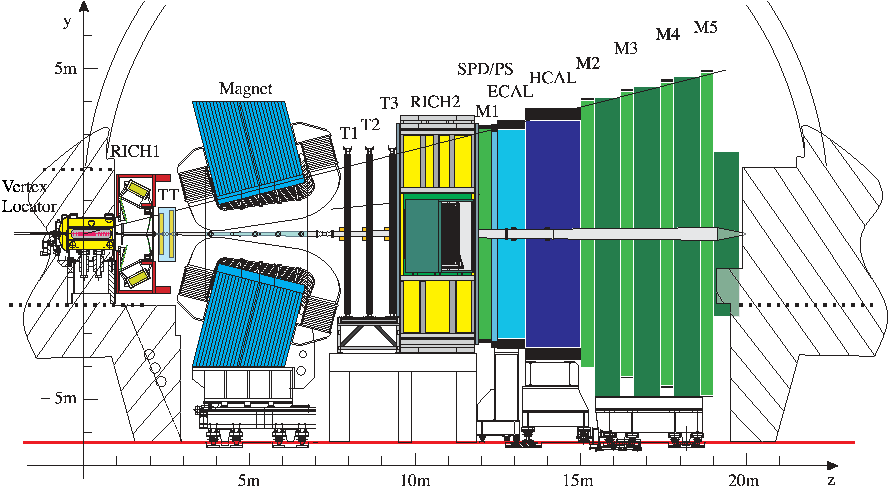
\includegraphics[width=0.8\textheight]{lhcb-detector-cross-section}
%  \caption[Cross-section view of \LHCb, cut in the non-bending $y$--$z$ plane]%
%    {Cross-section view of \LHCb, cut in the non-bending $y$--$z$ plane.}
%  \label{fig:LHCbCrossSection}
%  \end{center}
%\end{sidewaysfigure}



\chapter{Selection of neutrino interactions in the ECal}
\label{chap:NeutrinoInteractionSelection}
This analysis presents a measurement of the CC inclusive interaction cross-section of $\nu_\mu$ with lead nuclei using the ND280 tracker ECals.  To make such a measurement, a sample of neutrino interaction vertices within the ECal must be found.  The selection of events is based on the enhanced reconstruction outlined in chapter~\ref{chap:EnhancedECalReconstruction}.  However, as described in section~\ref{sec:ReconOutput}, the output of the enhanced reconstruction has been kept generic and isn't specifically tailored to this task.  The reconstruction's outputs a set of clusters which contain a set of 3D tracks and every pairwise crossing that said tracks make.  While it is true that in some situations the reconstruction will accurately represent a vertex out of the box, e.g. when only two tracks are reconstructed in the cluster, there will be many situations where extra reconstruction steps are needed before any further selection can take place.  After the final reconstruction steps have been discussed, a full discussion of the neutrino selection follows.

\section{Vertex reconstruction}
\label{sec:VertexReconstruction}
The output of the enhanced reconstruction already supplies most of the necessary information to reconstruct vertices in the ECal.  As a reminder, the reconstruction outputs a set of ECal clusters which contain the following:
\begin{itemize}
  \item A set of 3D reconstructed tracks
  \item The position at which every pairwise combination of 3D tracks most closely cross (pairwise crossings)
\end{itemize}
The reconstruction makes no quality checks on the 3D tracks in each cluster.  So, the first step is to remove any poorly reconstructed tracks from the cluster.  The need for this step is shown in Fig.~\ref{fig:AngularSeparationNoRejection} which shows the angular separation of reconstructed tracks with the simulated particle which created them, taken from beam Monte Carlo.  While the majority of tracks generally have a small angular separation, Fig.~\ref{fig:AngularSeparationNoRejection} clearly shows a build up of tracks which are offset by 90$^\circ$ to the simulated particles.
\newline
\newline
\begin{figure}%
  \centering
  \subfloat[No track rejection.]{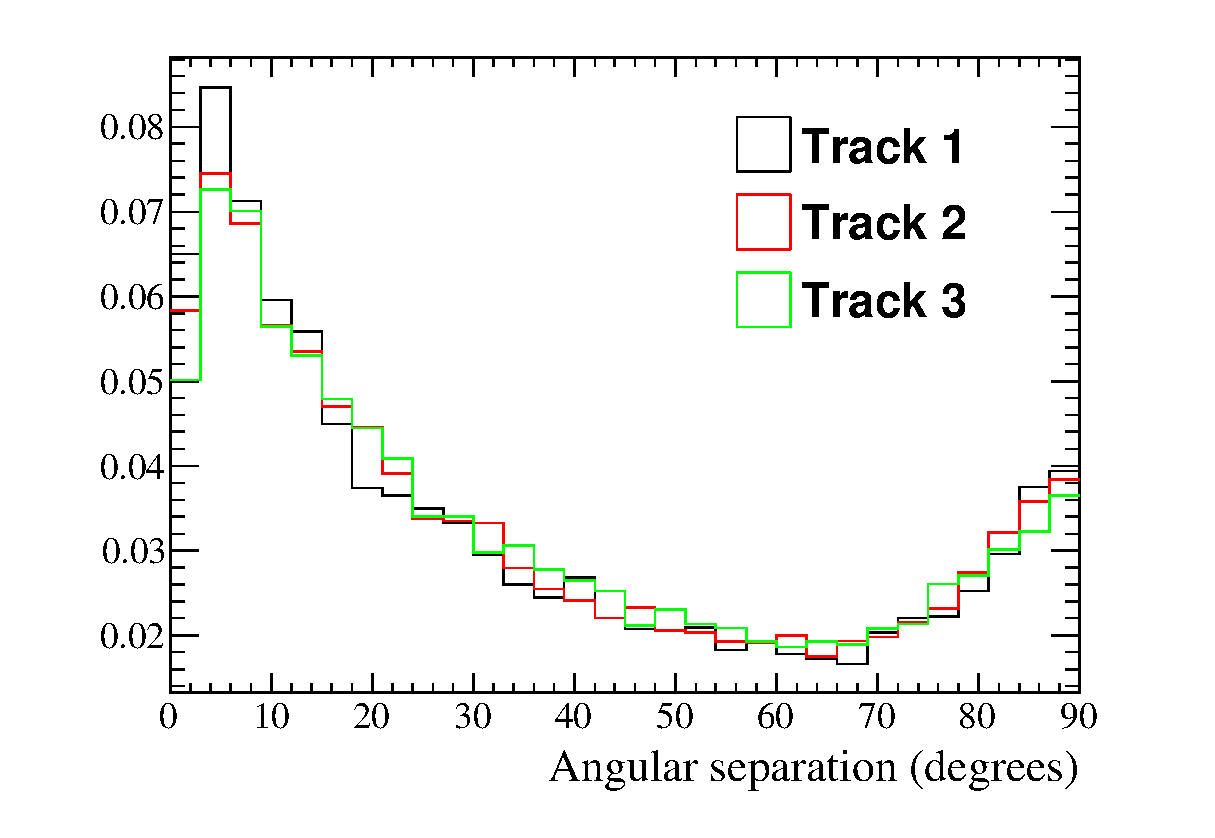
\includegraphics[width=9cm]{images/selection/track_rejection/AngularSeparationNoRejection} \label{fig:AngularSeparationNoRejection}}
  \subfloat[With track rejection.]{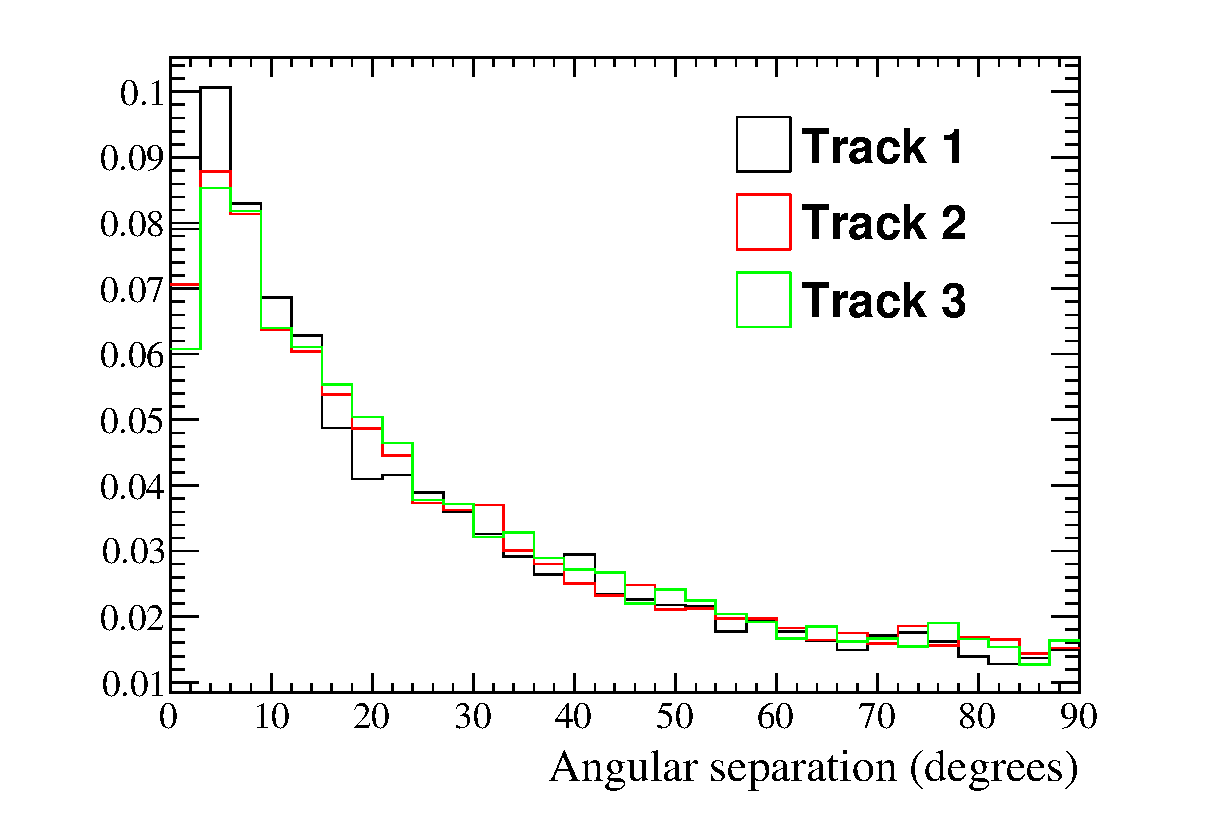
\includegraphics[width=9cm]{images/selection/track_rejection/AngularSeparationWithRejection}\label{fig:AngularSeparationWithRejection}}
  \caption{Angular separation of the reconstructed tracks in an ECal cluster with the beam-simulated particle that created them.  The black, red and green histograms are the tracks that were reconstructed first, second and third respectively.  All histograms are area normalized.}
  \label{fig:TrackRejectionAngularSeparation}
\end{figure}
There are two catagories of bad track reconstruction.  The first is where the 3D matching matches two 2D tracks which do not have sufficient information to fully model a 3D track.  Specifically, one of the 2D tracks involved in the matching only uses one ECal layer.  As the 3D track reconstruction requires information from both ECal views, tracks which fall into this catagory do not supply enough information to reconstruct a good quality track.  The second catagory is where the 3D matching produces a grossly incorrect match.  The matcher is designed to continually match 2D tracks together until no more 2D tracks are left in the matching pool.  So, there are situations where the last possible match made is in no way suitable.  This situation is easily indentified by matched 2D tracks which do not overlap.  For example, one of the 2D tracks uses layers 16, 18 and 20 and the other 2D track uses layers 1 and 3.  By removing these two types of tracks from the cluster, the 90$^\circ$ build up in the angular separation distribution is surpressed, as shown in Fig.~\ref{fig:AngularSeparationWithRejection}.  By removing these catagories of tracks, approximately 22$\%$ of tracks are rejected.
\newline
\newline
The final states of a neutrino interaction originate from the same point in space.  So, assuming that the reconstructed tracks represent the final states, the reconstructed tracks should most closely cross at the point of interaction.  As stated above, one of the outputs of the reconstruction are the pairwise crossings of the constituent tracks in the ECal cluster.  Using the above assumptions,  the pairwise crossings should be in close proximity to one another when the reconstructed tracks represent the final states of an interaction.  This idea promotes a relatively simple method of vertex reconstruction: attempt to cluster the pairwise crossings together if the pairwise crossings are in close proximity.  To quantatively define this proximity, the quality of the pairwise crossing also has to be considered.
\newline 
\newline
As with the 3D tracks, the reconstruction does not perform any quality checks on the pairwise crossings of the tracks.  As the reconstruction will always find a crossing location for a pair of 3D tracks, some of the pairwise crossings will not represent anything physical.  The quality definition chosen is simple: pairwise crossings are defined as bad if the crossing location is far away from either of the tracks it is associated with.  However, the distance definition is not trivial to define and should be closely correlated with the vertex reconstruction method.  For example, a two track vertex would provide very little constraint on the distance which defines a bad crossing, whereas a three track vertex may provide a bad crossing distance constraint which is too strict and destroys the majority two track vertices. 
\newline
\newline
The above discussion promotes two parameters which will govern the vertex reconstruction: the required proximity of two crossings to be clustered together, $d_c$, and the distance of a crossing from its constituents tracks to be classified as bad quality, $d_q$.  To quantify these values, a sample of reconstructed events matched to interactions in the ECals are used which are taken from beam Monte Carlo.  The reconstruction (the pairwise crossing rejection and clustering) is repeatedly run over the sample for different values of the $d_c$ and $d_q$ to find the optimum values.  To define the optimum value, a figure of merit is necessary.  After running the reconstruction for a given $d_c$ and $d_q$, the number vertices are separated into one, two and three track vertices and the true neutrino interactions which created the reconstructed vertices are associated.  A reconstructed vertex is tagged as correctly reconstructed if it contains the same number of reconstructed tracks as the number of charged final states in the associated neutrino interaction.  By defining the number of correctly reconstructed one, two and three track vertices as $N_1$, $N_2$ and $N_3$ respectively, the figure of merit, $\phi^{\textrm{vertices}}$, is
\begin{equation}
  \phi^{\textrm{vertices}} = N_1N_2N_3.
\end{equation}
\begin{figure}
  \centering
  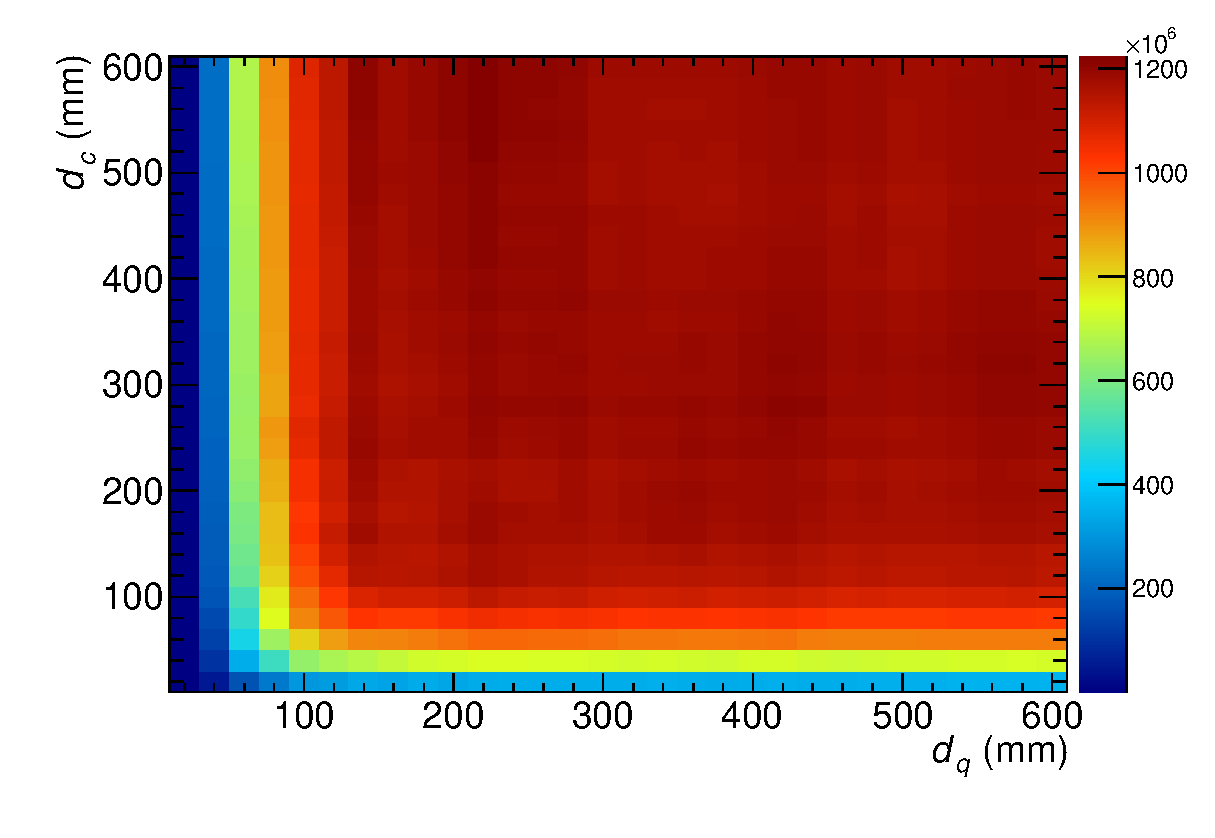
\includegraphics[width=12cm]{images/selection/vertex_recon/FOM_2D}
  \caption{Values of $\phi^{\textrm{vertices}}$ in ($d_q$,$d_c$) space.  The colour corresponds to the magnitude of $\phi^{\textrm{vertices}}$.}
  \label{fig:VertexReconFOM}
\end{figure}
\begin{figure}
  \centering
  \subfloat[$d_q$]{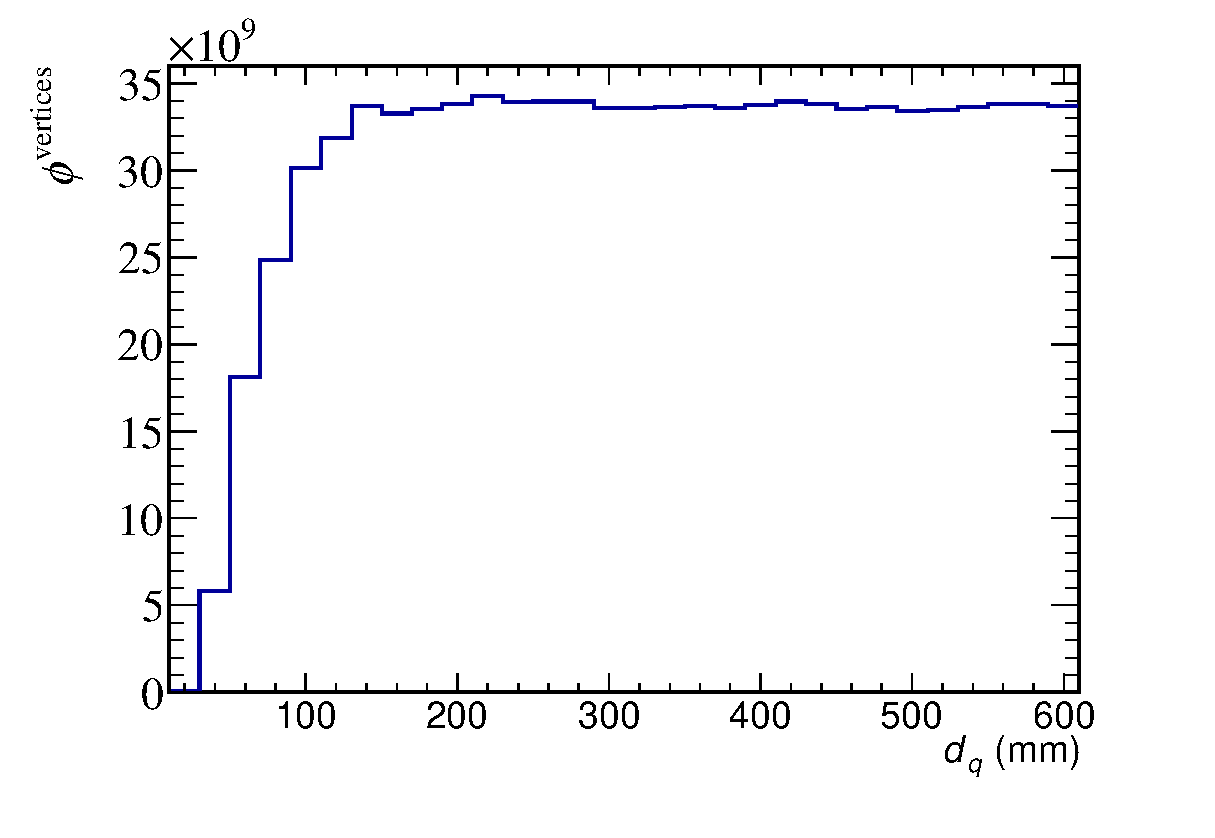
\includegraphics[width=9cm]{images/selection/vertex_recon/dq_marginalize} \label{fig:dqMarginalize}}
  \subfloat[$d_c$]{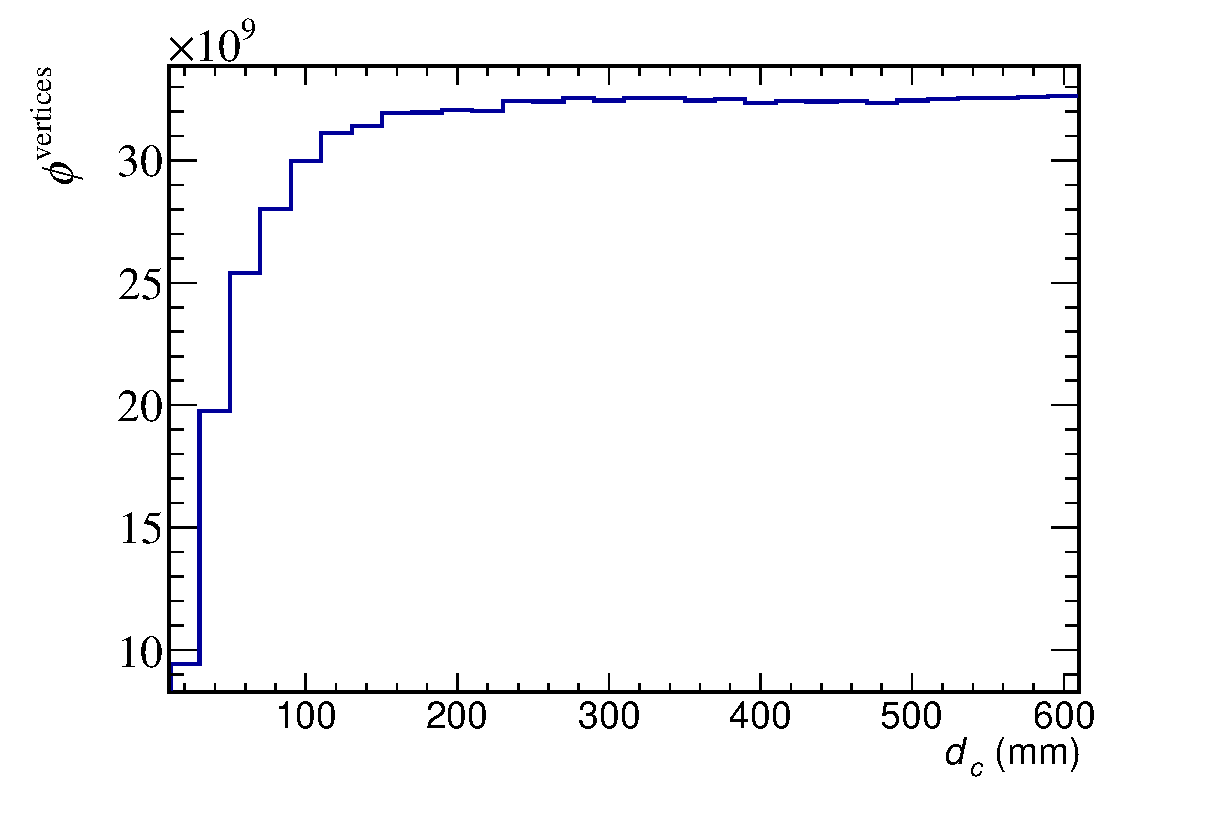
\includegraphics[width=9cm]{images/selection/vertex_recon/dc_marginalize} \label{fig:dcMarginalize}}
  \caption{$\phi^{\textrm{vertices}}$ vs the marginalized vertex reconstruction parameters.}
  \label{fig:VertexReconMarginalizedDistributions}
\end{figure}
By mapping out $\phi^{\textrm{vertices}}$ in ($d_q$,$d_c$) space, information about the preferred values of $d_q$ and $d_c$ can be found.  This space is shown in Fig.~\ref{fig:VertexReconFOM}.  It is clear from Fig.~\ref{fig:VertexReconFOM} that there is no clear maximum, but rather a plateau of  $\phi^{\textrm{vertices}}$ for $d_q$ and $d_c$ greater than 140 mm.  So, marginalized distributions of $d_q$ and $d_c$ can be produced to find where $\phi^{\textrm{vertices}}$ approaches zero which are shown in Fig.~\ref{fig:dqMarginalize} and Fig.~\ref{fig:dcMarginalize} respectively.  The values chosen are shown in table~\ref{table:VertexReconParameters}. 
\begin{table}[b!]
  \begin{tabular}{ c c }
    $\phi_d$ & $\phi_c$ \\ \hline \hline
    $<$ 140 mm & $<$ 200 mm \\
  \end{tabular}
  \caption{Parameters for the vertex reconstruction in the ECal.}
  \label{table:VertexReconParameters}
\end{table}
The reconstruction now assesses the quality the crossings and then attempts to cluster the good quality crossings together to form vertex candidates.  The final step is to use the constituent tracks of each vertex candidate in a fit to estimate the position of the vertex.  The following method was proposed by X. Lu.  The position of the vertex, $\vec{P}$, is defined such that the sum of the squares of the distance of each track to $\vec{P}$ is minimised.  An example setup of this is shown in Fig.~\ref{fig:VertexVectorDiagram} for three constituent tracks.  By defining the square of the of the distance of a line, $l_i$, to $\vec{P}$ as $|\vec{r}_i|^2$, the function to minimise is
\begin{figure}[!b]
  \centering
  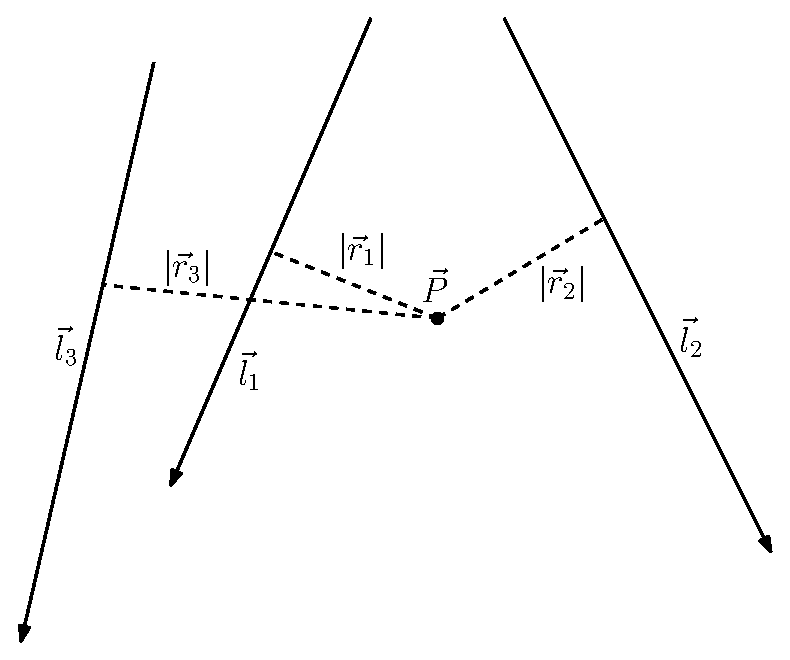
\includegraphics[width=8cm]{images/selection/vertex_recon/vertex_vector_diagram}
  \caption{Example of the vertex position, $\vec{P}$ for three lines: $\vec{l}_1$, $\vec{l}_2$ and $\vec{l}_3$. $|\vec{r}_1|$, $|\vec{r}_2|$ and $|\vec{r}_3|$ are the perpendicular distances of $\vec{l}_1$, $\vec{l}_2$ and $\vec{l}_3$ to $\vec{P}$ respectively.}
  \label{fig:VertexVectorDiagram}
\end{figure}
\begin{equation}
  D = \sum_i |\vec{r}_i|^2.
  \label{eqn:SumOfSquares}
\end{equation}
$\vec{P}$ is then defined as the point in space which satisfies
\begin{equation}
  \frac{\partial D}{\partial x} = \frac{\partial D}{\partial y} = \frac{\partial D}{\partial z} = 0.
  \label{eqn:SumOfSquaresMinCondition}
\end{equation}
The value of $|\vec{r}_i|$ is trivially defined by simple vector properties as 
\begin{equation}
  |\vec{r}_i| = \frac{|(\vec{P} - \vec{a}_i) \cross \vec{v}_i|}{|\vec{v}_i|} = |(\vec{P} - \vec{a}_i) \cross \hat{v}_i|,
  \label{eqn:DistanceOfPointToLine}
\end{equation}
where $\vec{v}_i$ is the direction vector of $\vec{l}_i$ and $\vec{a}_i$ is a point along $\vec{l}_i$.  By defining $\vec{P}$ mathematically as
\begin{equation}
  \vec{P} = x\hat{\imath} + y\hat{\jmath} + z\hat{k},
  \label{eqn:PDefinition}
\end{equation}
equation~\ref{eqn:SumOfSquaresMinCondition} can be solved.  The following derivation is only for $\partial D/\partial x$ as the method is identical for $\partial D/\partial x$, $\partial D/\partial y$ and $\partial D/\partial z$.
\begin{eqnarray}
  \frac{\partial D}{\partial x} & = & \sum_i 2\vec{r}_i \cdot \frac{\partial \vec{r}_i}{\partial x} \\
  & = & 2\sum_i \big[(\vec{P} - \vec{a}_i) \cross \hat{v}_i\big] \cdot \big[\hat{\imath} \cross \hat{v}_i\big] \nonumber \\
  & = & 2x \sum_i (\hat{\imath} \cross \hat{v}_i) \cdot ( \hat{\imath} \cross \hat{v}_i) + 2y \sum_i (\hat{\jmath} \cross \hat{v}_i) \cdot ( \hat{\imath} \cross \hat{v}_i) + 2z \sum_i (\hat{k} \cross \hat{v}_i) \cdot ( \hat{\imath} \cross \hat{v}_i) \nonumber \\
  &\qquad & - 2(\vec{a}_i \cross \hat{v}_i) \cdot ( \hat{\imath} \cross \hat{v}_i). \nonumber
  \label{eqn:dDdxDerivation}
\end{eqnarray}
By applying the same steps for $\partial D/\partial y$ and $\partial D/\partial z$, the matrix equation
\begin{equation}
%  \[ \left( \begin{array}{ccc}
%      0 & 0 & 0 \\
%      0 & 0 & 0 \\
%    0 & 0 & 0 \end{array} \right)\]
%  \label{eqn:VertexReconMatrix}
  \begin{pmatrix}
    \displaystyle\sum_i [\hat{\imath} \cross \hat{v}] \cdot (\hat{\imath} \cross \hat{v}) & \displaystyle\sum_i [\hat{\jmath} \cross \hat{v}] \cdot (\hat{\imath} \cross \hat{v}) & \displaystyle\sum_i [\hat{k} \cross \hat{v}] \cdot (\hat{\imath} \cross \hat{v}) \\
    \displaystyle\sum_i [\hat{\imath} \cross \hat{v}] \cdot (\hat{\jmath} \cross \hat{v}) & \displaystyle\sum_i [\hat{\jmath} \cross \hat{v}] \cdot (\hat{\jmath} \cross \hat{v}) & \displaystyle\sum_i [\hat{k} \cross \hat{v}] \cdot (\hat{\jmath} \cross \hat{v}) \\ 
    \displaystyle\sum_i [\hat{\imath} \cross \hat{v}] \cdot (\hat{k} \cross \hat{v}) & \displaystyle\sum_i [\hat{\jmath} \cross \hat{v}] \cdot (\hat{k} \cross \hat{v}) & \displaystyle\sum_i [\hat{k} \cross \hat{v}] \cdot (\hat{k} \cross \hat{v}) 
  \end{pmatrix}
  \begin{pmatrix}
   x \\
   y \\
   z
  \end{pmatrix}
  =
  \begin{pmatrix}
    \displaystyle\sum_i [\vec{a}_i \cross \hat{v}] \cdot (\hat{\imath} \cross \hat{v}) \\
    \displaystyle\sum_i [\vec{a}_i \cross \hat{v}] \cdot (\hat{\jmath} \cross \hat{v}) \\
    \displaystyle\sum_i [\vec{a}_i \cross \hat{v}] \cdot (\hat{k} \cross \hat{v})
  \end{pmatrix}
  \label{eqn:VertexReconMatrix}
\end{equation}
can be built up.  By defining the equation~\ref{eqn:VertexReconMatrix} as
\begin{equation}
  \underline{\underline{A}} \vec{P} = \vec{B},
  \label{eqn:VertexReconMatrixSimple}
\end{equation}
where $\underline{\underline{A}}$ is the matrix on the left hand side of equation~\ref{eqn:VertexReconMatrix} and $\vec{B}$ is the vector on the right hand side of equation~\ref{eqn:VertexReconMatrix}.  $\vec{P}$ is finally
\begin{equation}
  \vec{P} = \underline{\underline{A}}^{-1} \vec{B}.
  \label{eqn:VertexReconMatrixSolution}
\end{equation}
While the inversion of $\underline{\underline{A}}$ is in principle analytically solvable, it was decided that the inversion would be handled numerically.  So, to find $\vec{P}$, the vertex reconstruction builds $\underline{\underline{A}}^{-1}$ (by building and inverting $\underline{\underline{A}})$ and $\vec{B}$ and then applies equation~\ref{eqn:VertexReconMatrixSolution}.
\newline
\newline
By applying the steps outlined above to every reconstructed ECal cluster, a set of candidate vertices are formed.  As the enhanced reconstruction is only capable of reconstructing straight tracks, bending trajectories tend to be reconstructed as two or more tracks.  The crossings associated with such tracks can, and do, pass the vertex reconstruction criteria defined in table~\ref{table:VertexReconParameters}.  An extreme example of this topology is shown in Fig.~\ref{fig:TrackMergingEventDisplay} in which a curving $\mu^-$ is reconstructed as four tracks.  So, the final step on the reconstruction is to attempt to merge tracks to model the curving trajectory topology.  Firstly, the reconstructed crossings associated with a clean curving trajectory should pass the crossing quality cut but should be sufficiently far away from any other crossing that it is not clustered during the vertex clustering stage.  Therefore, track merging candidates can be initially identified by searching for reconstructed vertices with exactly two track constituents.  As an example, all three of the crossings shown in Fig.~\ref{fig:TrackMergingEventDisplay} are correctly identified by this check.  The two constituent tracks of the identified vertex will form the merged track, so the reconstruction checks the shape that the merged track would make against a set of conditions to decide if the merging should be performed. 
\begin{figure}
  \centering
  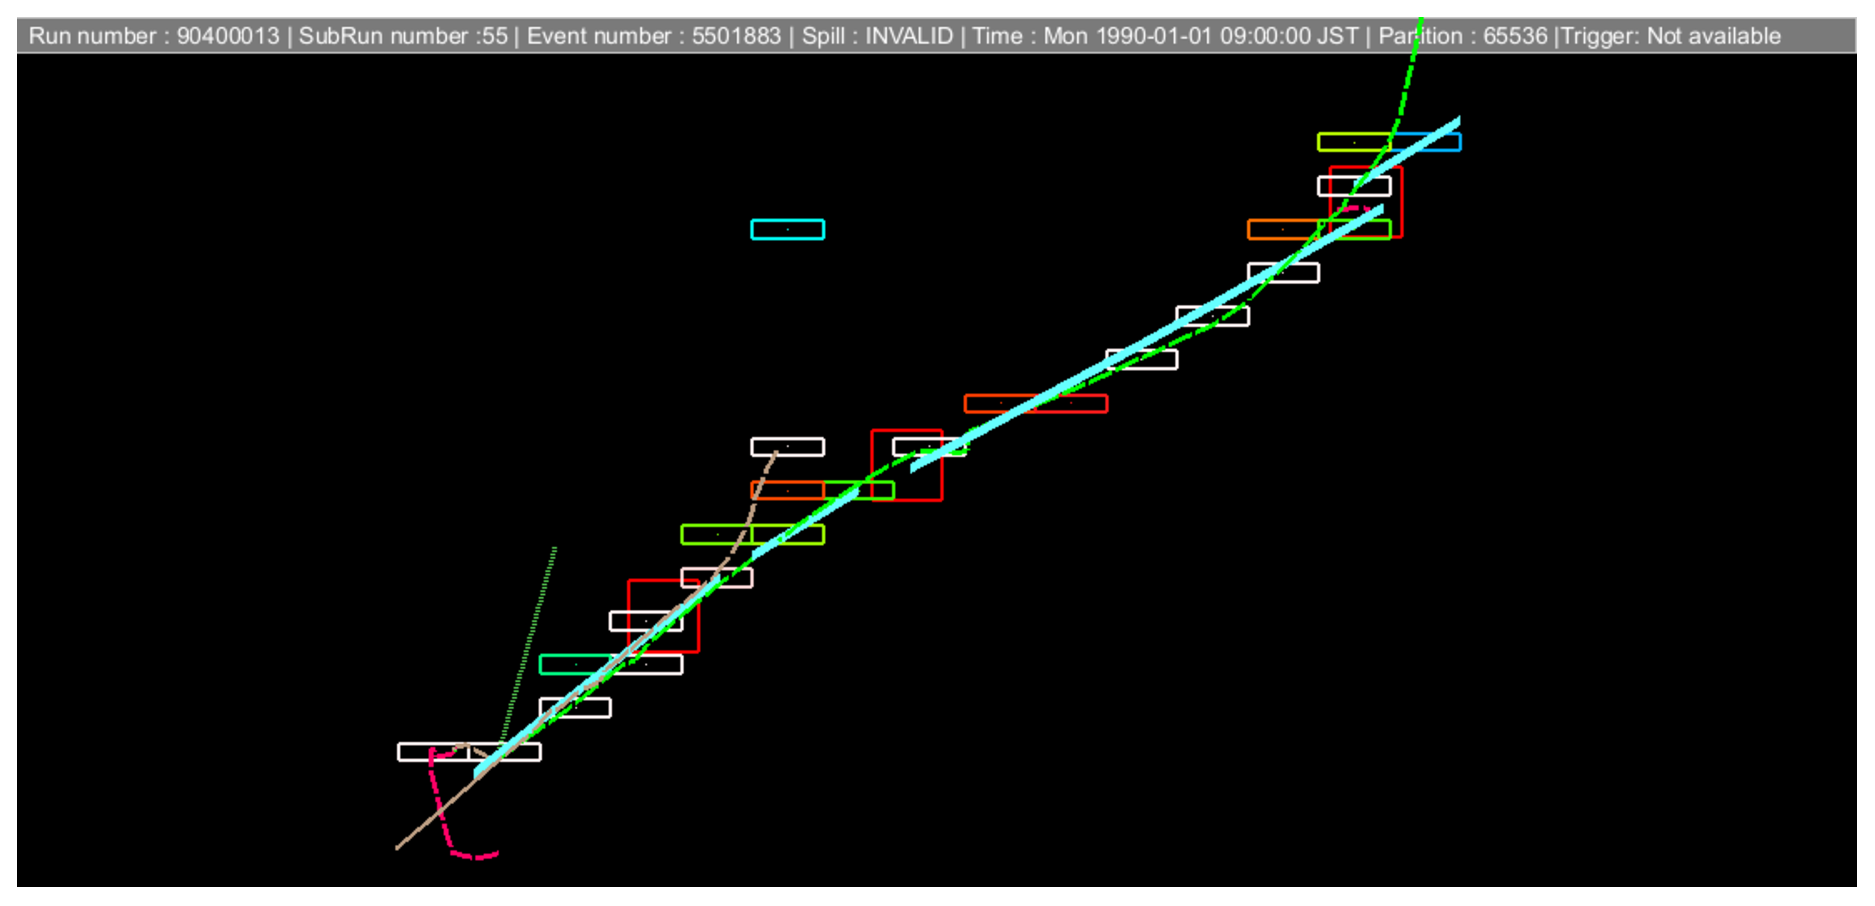
\includegraphics[width=12cm]{images/selection/vertex_recon/track_merging_event_display.eps}
  \caption{Example event display showing a track merging candidate.  The final state $\mu^-$ (in green) curves in a complicated way and is reconstructed as four tracks (in light blue).  The pairwise crossings of the reconstructed tracks are the red squares.  The muon is produced by a charged current interaction in the top left barrel ECal producing two $\pi^+$ (in brown) and the curving $\mu^-$. }
  \label{fig:TrackMergingEventDisplay}
\end{figure}
To identify and tune the condtitions for merging tracks, two metrics are used.  The first metric is used for identification of the merging conditions and uses the truth information provided by the geant4 simulation.  For every two track vertex that was formed by the vertex clustering, the simulated particle that produced each of the two constituent tracks was checked.  If the sample particle is matched to both tracks, then the merging candidate is tagged as a correct match, otherwise it is tagged as an incorrect match.  The second metric is used for tuning the identified merging conditions.  As part of this analysis is a search for neutrino intercations using vertex-based reconstruction, there will be an expected loss of signal by track merging which must be minimised.  So, the track merging condition tuning should be based on ECal signal interactions.  As described above, the only tracks that are proposed as merging candidates are those which are constituents of a two track vertex.  So, the track merging tuning attempts to separate signal and background events which are reconstructed as a vertex with two track constituents.  It is preferrable that the merging choses quality over quality so the tuning figure of merit is defined as 
\begin{equation}
  \phi^{\textrm{merge}} = \epsilon \eta^2
  \label{eqn:TrackMergingTuningMetric}
\end{equation}
where $\epsilon$ is the efficiency of the track merging to keep signal events reconstructed as two track vertices and $\eta$ is the purity of the events that remain as two track vertices after merging has taken place.
\newline
\newline
The first merging condition identified is the cosine of the opening angle, $\cos\theta$, subtended by the two constituent tracks bounded between 0 and 1 which is shown in Fig.~\ref{fig:TrackMergingConditionCosTheta}.  The opening angle is clearly a powerful discriminator.  The distribution for incorrect matches is very flat across the full angular range whereas there is a clear build up correct matches as $\cos\theta \rightarrow 1$.
\begin{figure}[!b]
  \centering
  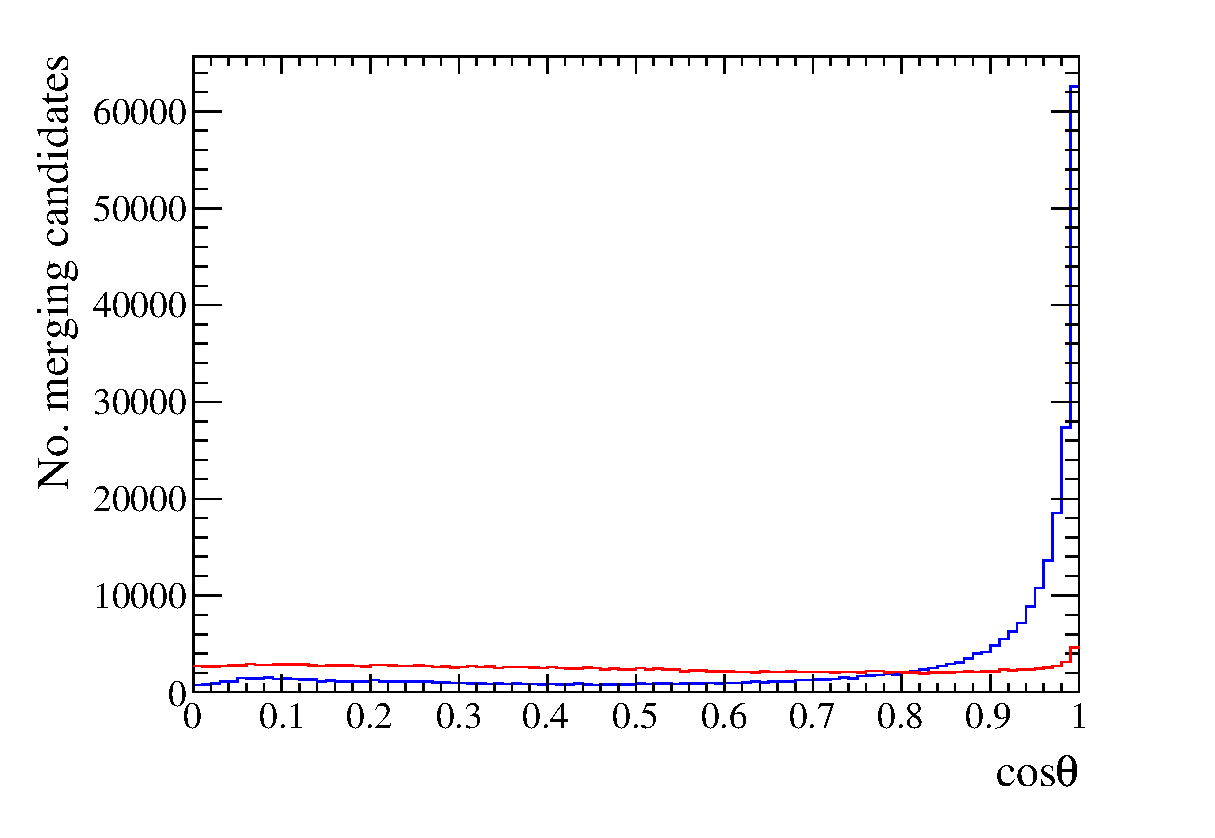
\includegraphics[width=10cm]{images/selection/vertex_recon/merging_candidates_cos_theta}
  \caption{The cosine of the angle subtended by the merging candidates, bounded between 0 and 1. The correct matches and incorrect matches are the blue and red histograms respectively.}
  \label{fig:TrackMergingConditionCosTheta}
\end{figure}
\newline
\newline
The second merging condition identified, called 'distance ratio', measures the ratio of the distance between the two constituent tracks' closest points, $d^{\textrm{small}}$ to the distance between their furthest points, $d^{\textrm{large}}$.  An example of how $d^{\textrm{small}}$ and $d^{\textrm{large}}$ are calculated is shown in Fig.~\ref{fig:DistanceRatioEventDisplay}.    
\begin{figure}[!b]
  \centering
  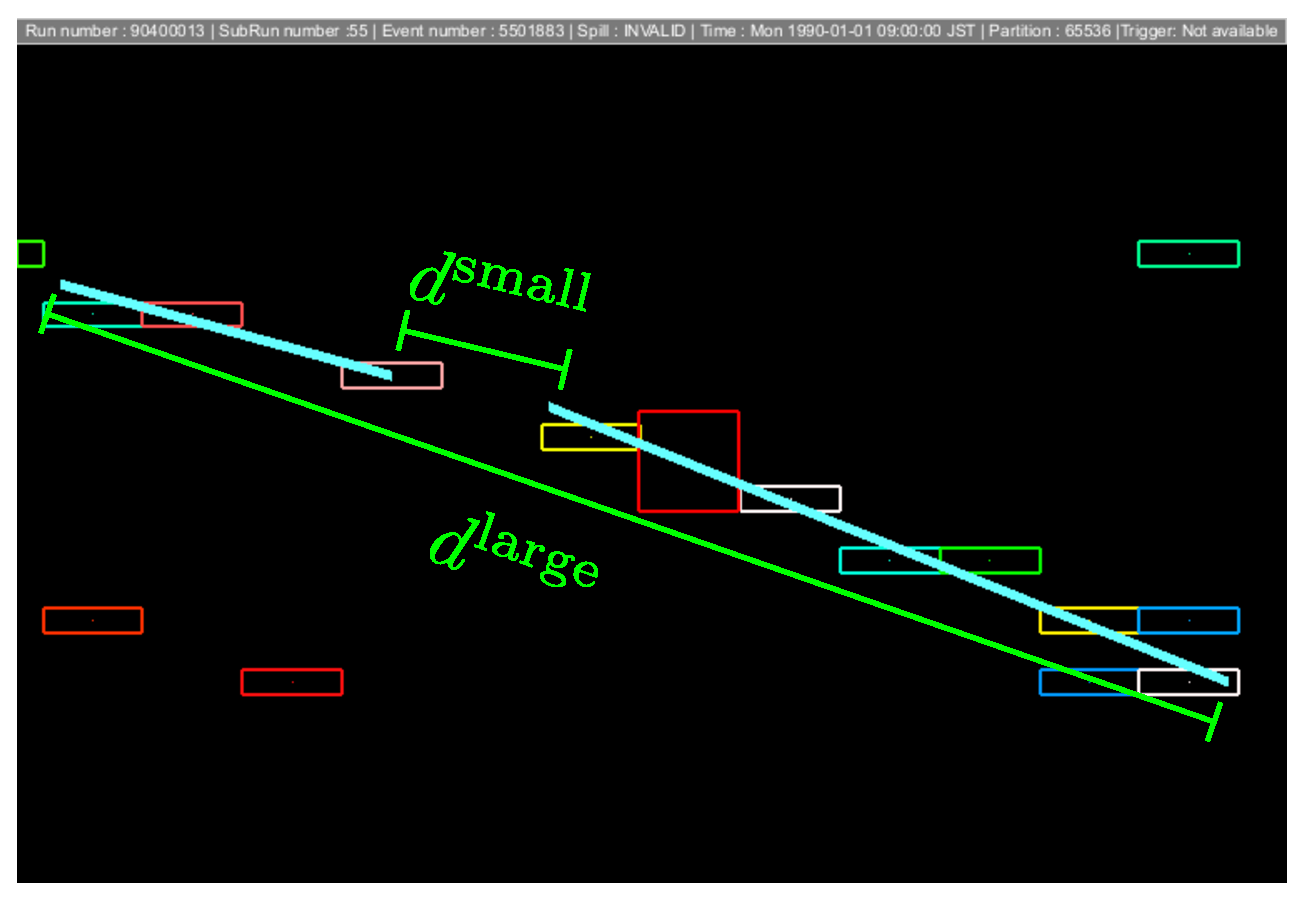
\includegraphics[width=10cm]{images/selection/vertex_recon/distance_ratio_event_display}
  \caption{Example event display showing how the parameters of the distance ratio are calculated.  The distance ratio is defined as $d^{\textrm{small}}/d^{\textrm{large}}$.  The blue lines are the two reconstructed tracks which form the merging candidate and the red square is the crossing location of those tracks.}
  \label{fig:DistanceRatioEventDisplay}
\end{figure}
The distance ratio distribution is shown Fig.~\ref{fig:TrackMergingConditionDistanceRatio}.  While it may seem that there is very little discrimination power present in the distance ratio distribution, there is an underlying dependency between the distance ratio and the opening angle subtended by the constituent tracks, which has already been identified as a merging condition.
\begin{figure}
  \centering
  \subfloat[No cuts applied.]{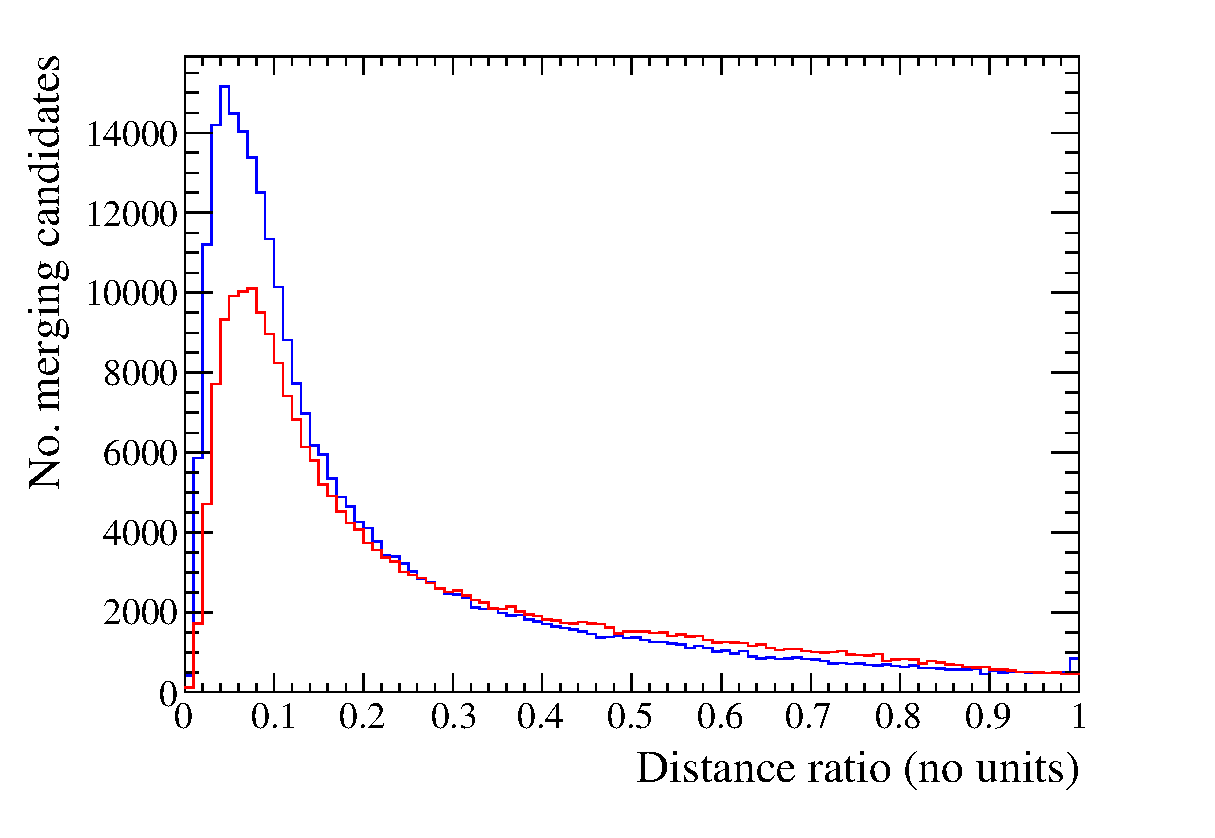
\includegraphics[width=9cm]{images/selection/vertex_recon/merging_candidates_distance_ratio.eps} \label{fig:TrackMergingConditionDistanceRatio}}
  \subfloat[For $\cos\theta > 0.8$.]{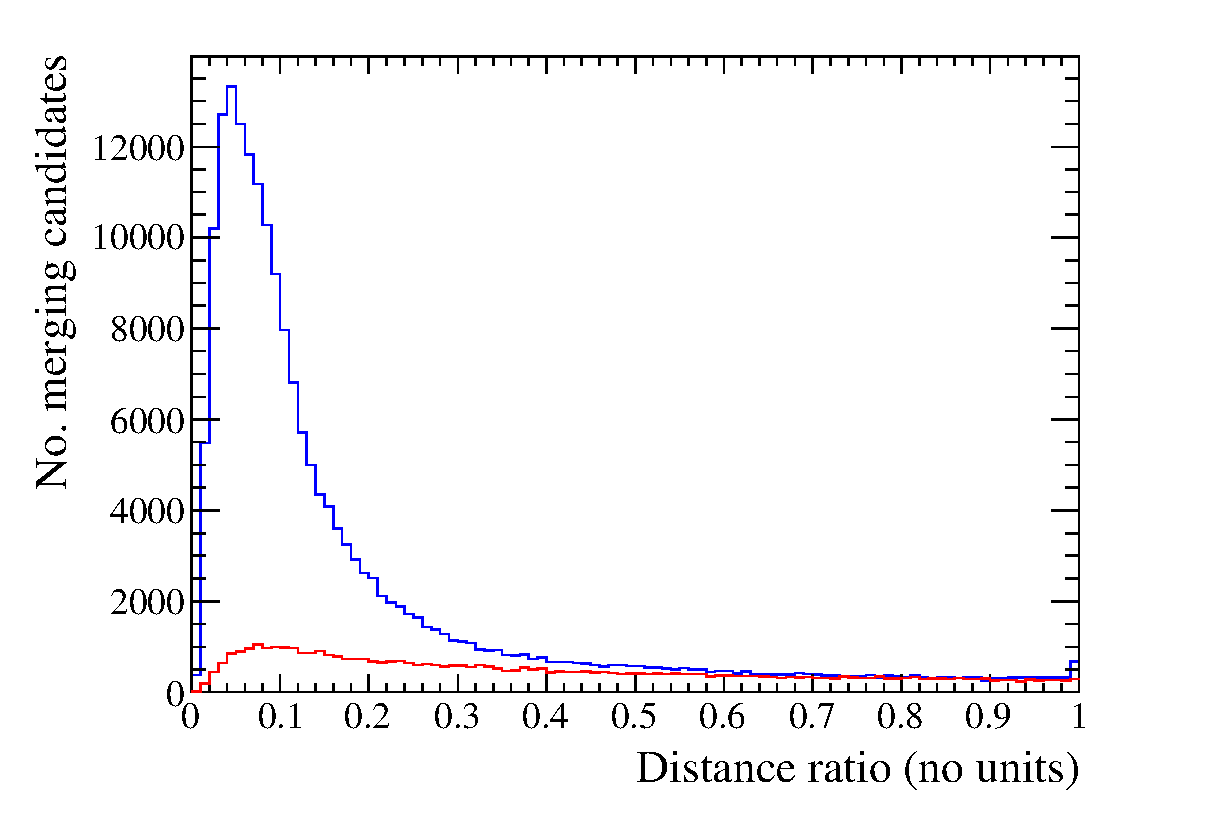
\includegraphics[width=9cm]{images/selection/vertex_recon/merging_candidates_distance_ratio_CosThetaGuessCut.eps} \label{fig:TrackMergingConditionDistanceRatioGuessCutCosTheta}}
  \caption{The distance ratio of the merging candidates.  The correct and incorrect matches are the blue and red histograms respectively.}
  \label{fig:TrackMergingConditionDistanceRatio}
\end{figure}
To illustrate this dependency two distributions are shown in Fig.~\ref{fig:TrackMergingConditionDistanceRatioVsCosTheta} which both show the distance ratio vs the cosine of the opening angle.  Fig.~\ref{fig:TrackMergingConditionDistanceRatioVsCosThetaCorrectMatch} only shows the correct matches and Fig.~\ref{fig:TrackMergingConditionDistanceRatioVsCosThetaIncorrectMatch} only shows the incorrect matches.  While it is true that there is a pileup of both correct matches and incorrect matches for low values of the distance ratio, the opening angle separates the two catagories out.  Specifically, the correct matches pileup occurs as $\cos\theta \rightarrow 1$ and the incorrect matches pileup occurs as $\cos\theta \rightarrow 0$.  To further illustrate this point, a new distance ratio distribution is shown in Fig.~\ref{fig:TrackMergingConditionDistanceRatioGuessCutCosTheta}, but with a $\cos\theta > 0.8$ guess cut applied.  Comparing the distributions shown in Fig.~\ref{fig:TrackMergingConditionDistanceRatio} and Fig.~\ref{fig:TrackMergingConditionDistanceRatioGuessCutCosTheta}, the effect of the $\cos\theta$ cut can clearly be seen.  The original pileup of incorrect matches seen in Fig.~\ref{fig:TrackMergingConditionDistanceRatio} is now gone, leaving an essentially flat incorrect matches distribution in Fig.~\ref{fig:TrackMergingConditionDistanceRatioGuessCutCosTheta} while leaving the correct matches structure intact.  
\begin{figure}
  \centering
  \subfloat[Correct matches only]{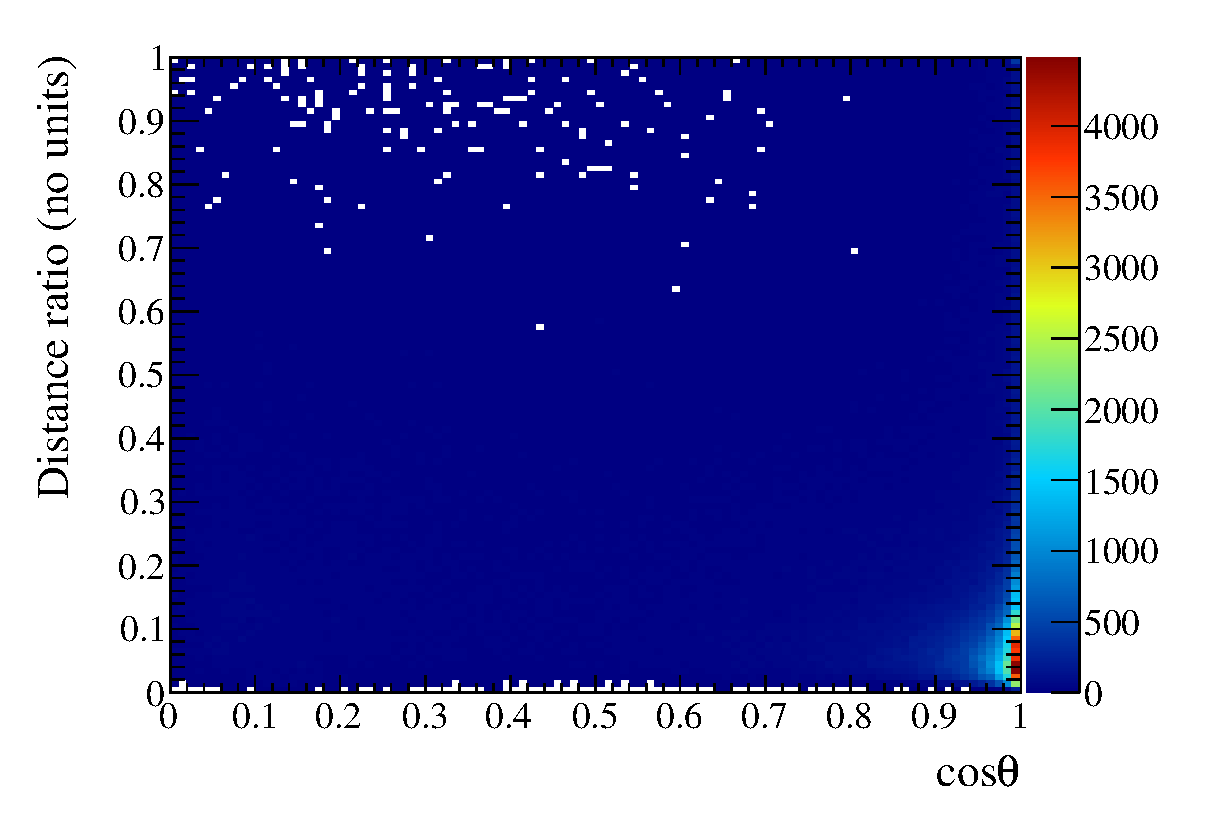
\includegraphics[width=9cm]{images/selection/vertex_recon/correct_merging_candidates_distance_ratio_vs_cos_theta.eps} \label{fig:TrackMergingConditionDistanceRatioVsCosThetaCorrectMatch}}
  \subfloat[Incorrect matches only]{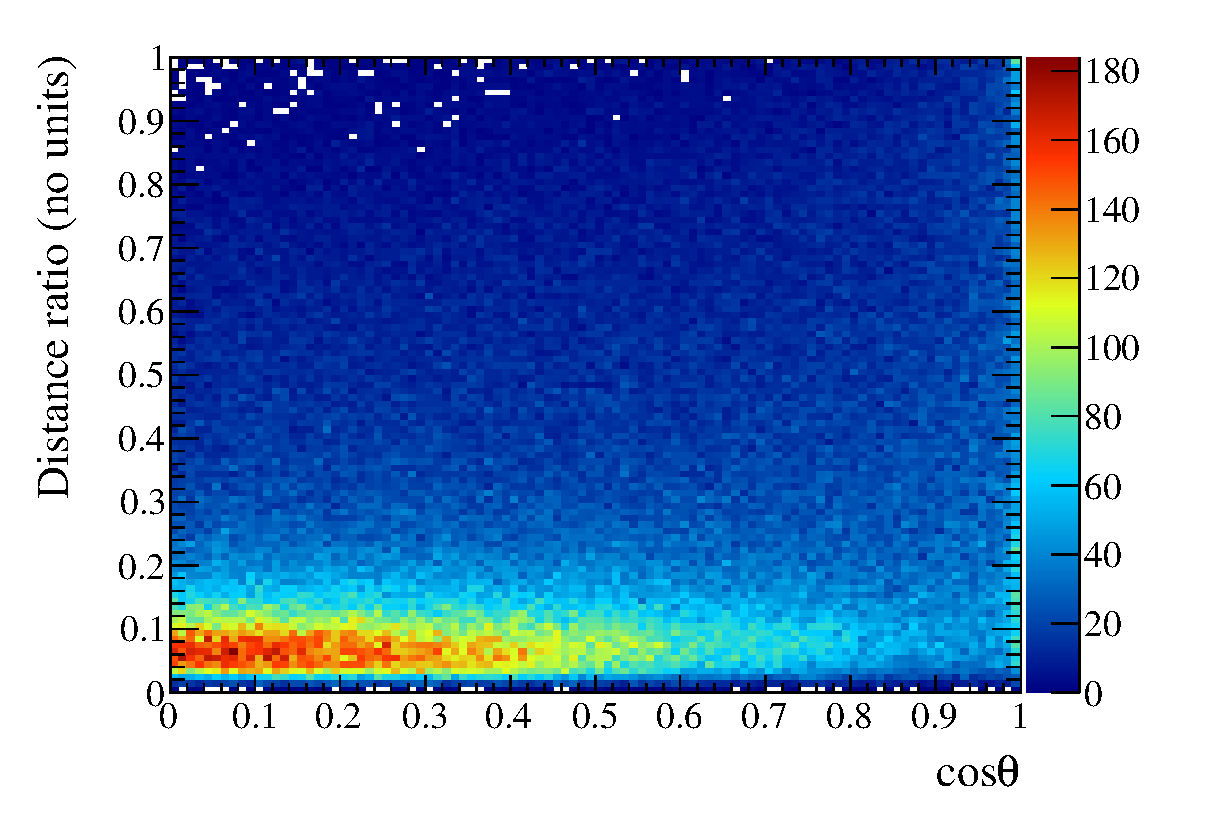
\includegraphics[width=9cm]{images/selection/vertex_recon/incorrect_merging_candidates_distance_ratio_vs_cos_theta.eps} \label{fig:TrackMergingConditionDistanceRatioVsCosThetaIncorrectMatch}}
  \caption{The distance ratio vs the cosine of the opening angle for track merging candidates.}
  \label{fig:TrackMergingConditionDistanceRatioVsCosTheta}
\end{figure}
\newline
\newline
By utilising both the distance ratio and $\cos\theta$ simultaneously, a better degree of separation can be found.  However care must be taken when tuning the distance ratio and $\cos\theta$ cuts to ensure optimal separation of signal and background is acheived.  It is clear from Fig.~\ref{fig:TrackMergingConditionCosTheta} and Fig.~\ref{fig:TrackMergingConditionDistanceRatioGuessCutCosTheta} that the correct matches pileup for low values of the distance ratio and high values of $\cos\theta$.  So events should only be tagged for merging when they have a distance ratio value lower than some threshold and a $\cos\theta$ value higher than some other threshold. To find these cut values, the track merging reconstruction was run multiple times, using different values of the thresolds for each run.  To take the dependency shown in Fig.~\ref{fig:TrackMergingConditionDistanceRatioVsCosTheta} into account, a square grid search in distance ratio and $\cos\theta$ space was used to find optimum cut values.  The tuning metric, as described in equation~\ref{eqn:TrackMergingTuningMetric}, was used to find the optimum cut values.
\begin{figure}[!b]
  \centering
  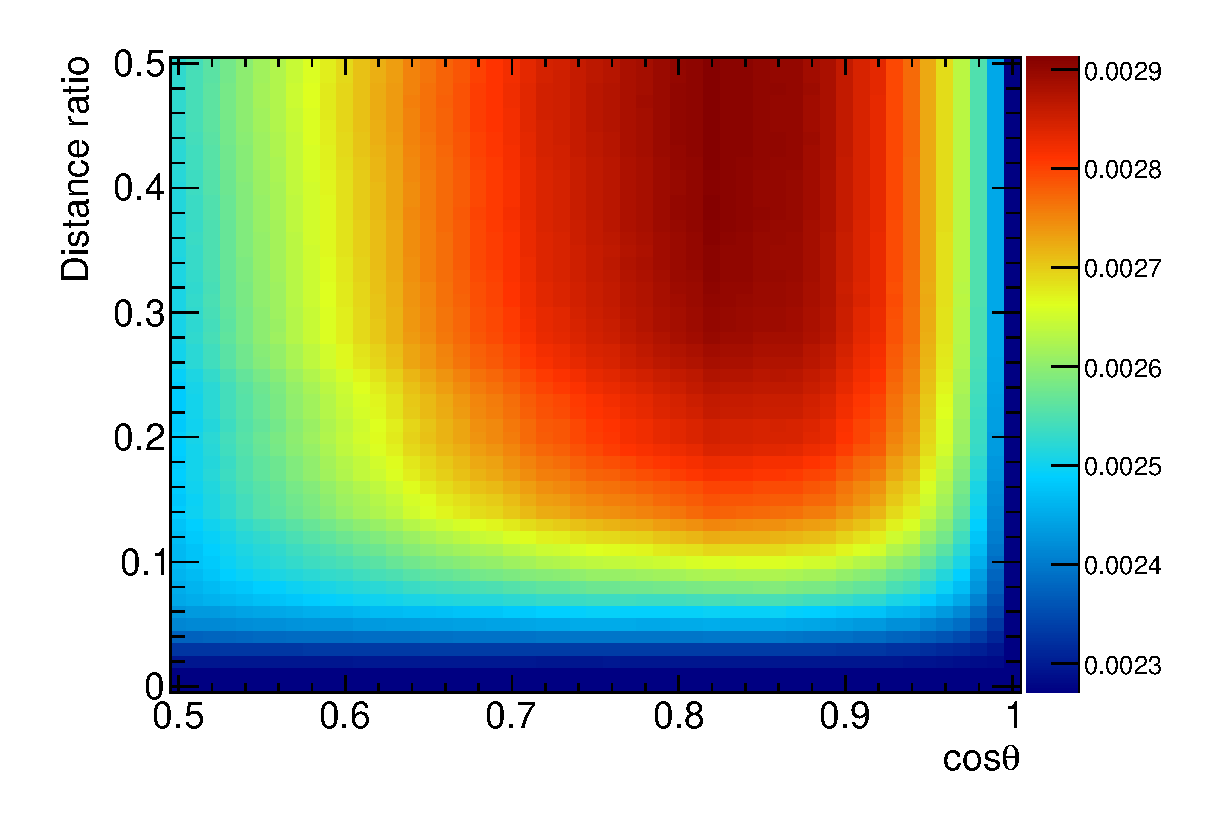
\includegraphics[width=10cm]{images/selection/vertex_recon/TrackMergingTuningFOM}
  \caption{Values of the tuning metric, as described in equation~\ref{eqn:TrackMergingTuningMetric}, in distance ratio cut vs $\cos\theta$ cut space.}
  \label{fig:TrackMergingTuningFOM}
\end{figure}
The tuning metric values in distance ratio cut vs $\cos\theta$ cut space are shown in Fig.~\ref{fig:TrackMergingTuningFOM}.  As was found in the tuning of the vertex clustering parameters, there is no clear maximum value of the tuning metric, but rather a plateau.  So, as was done in the vertex clustering tuning, marginalised distributions of tuning metric in distance ratio cut space and $\cos\theta$ cut space can be produced to find the optimum cut values. 
\begin{figure}
  \centering
  \subfloat[$d_q$]{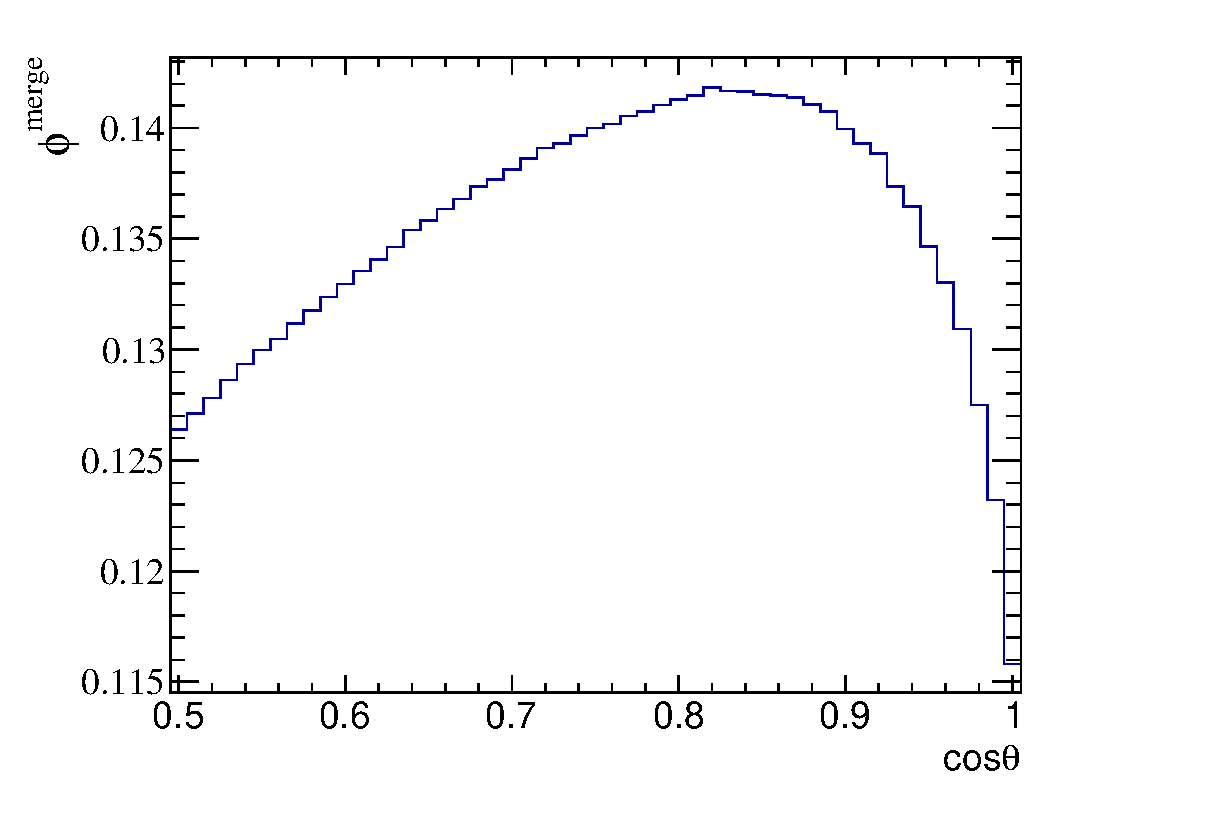
\includegraphics[width=9cm]{images/selection/vertex_recon/TrackMergingMarginalisedCosThetaFOM.eps} \label{fig:TrackMergingCosThetaMarginalize}}
  \subfloat[$d_c$]{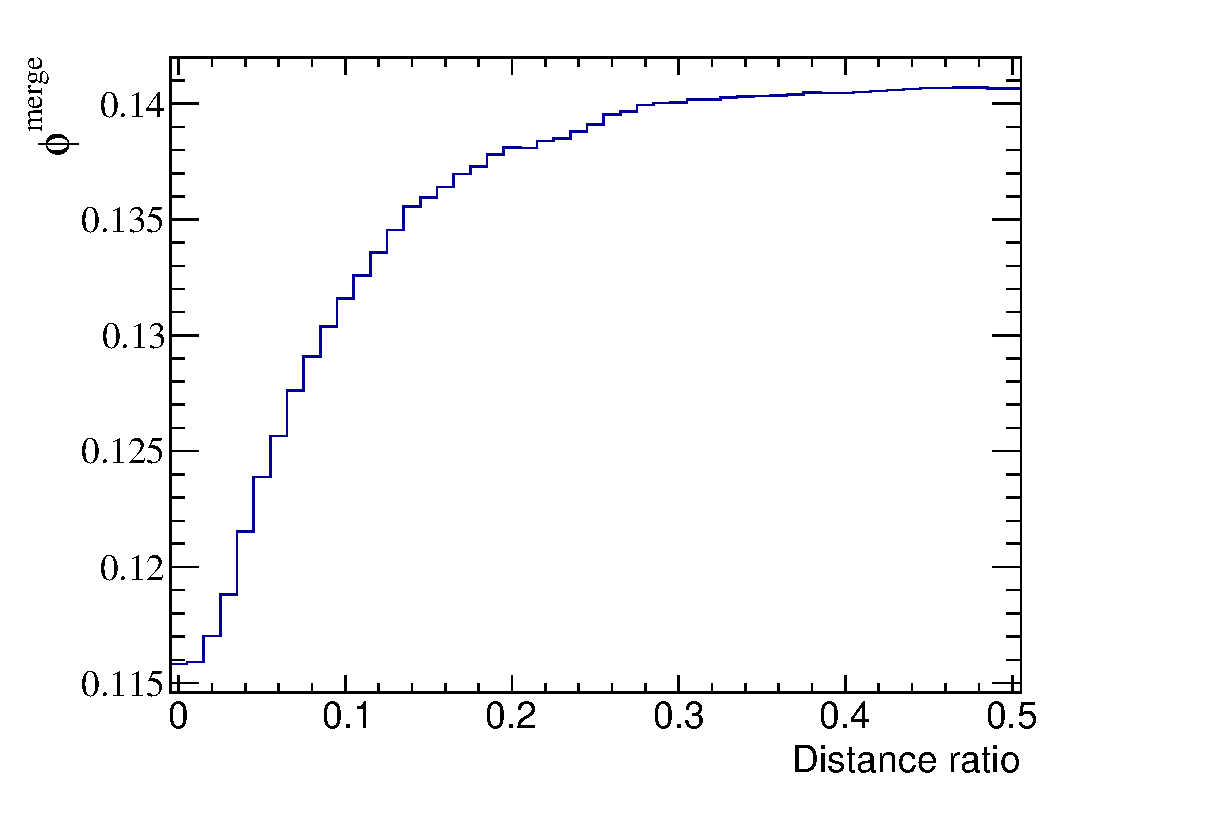
\includegraphics[width=9cm]{images/selection/vertex_recon/TrackMergingMarginalisedDistanceRatioFOM.eps} \label{fig:TrackMergingDistanceRatioMarginalize}}
  \caption{$\phi^{\textrm{merge}}$ vs the track merging conditions.}
  \label{fig:TrackMergingMarginalizedDistributions}
\end{figure}
The marginalised distributions for $\cos\theta$ and the distance ratio cuts are shown in Fig.~\ref{fig:TrackMergingCosThetaMarginalize} and Fig.~\ref{fig:TrackMergingDistanceRatioMarginalize} respectively.  In the case of the $\cos\theta$ cut there is a clearly preferred value, merging candidates should only be merged if $\cos\theta > 0.82$.  In the case of the distance ratio cut distribution, there is less of a clear maximum.  As the reconstruction is striving for quality over quantity, the cut value should be as close to the drop in $\phi^{\textrm{merge}}$.  It was decided that merging candidates should only be merged if the distance ratio is less than 0.32.
\begin{table}[b!]
  \begin{tabular}{ c c }
    $\cos\theta$ & Distance ratio \\ \hline \hline
    $>$ 0.82 & $<$ 0.32 \\
  \end{tabular}
  \caption{Cut values for the track merging in the ECal.}
  \label{table:VertexReconParameters}
\end{table}
The final identfied merging condition, called 'swing', measures 



%To identify which merging candidates should actually be matched together, the truth information from the simulation was used.  Specfically, merging candidates which should be matched together are found by checking which particle produced the two tracks.  If a single particle produced both tracks, then the merging candidate is tagged as signal, otherwise it is background.


%\section{Data selection}
%Data flags

\section{Monte Carlo selection}
Make the cuts

\section{Properties of events in selection}

